\chapter{Investment Algorithm}
\label{chapter:prospection}
Investing in a swarm is one of the key elements of the credit mining system. The investing module can be divided into two main stages, namely the \textit{prospecting} and \textit{mining} stage. After new swarm has been discovered, the credit mining system will estimate its return-of-investment potential on the \textit{prospecting stage}. Subsequently, in the \textit{mining stage}, the system will selectively join some of the high-prospected swarms to gain credits. The combination of both stages is the foundation of the whole investing algorithm. 

\section{Prospecting stage}
The cardinal problem of knowing a swarm's potential is to obtain reliable swarm size and piece availability information. That information is essential to predict future demand and estimate its return of investment. Given a large number of swarms, joining all of them is costly. Therefore, we introduce the \textit{prospecting algorithm}: a means to download a few pieces to roughly determine peers and piece information. Prospecting cost per swarm is limited, allowing us to estimate and compare the return-on-investment of a few thousand swarms easily.

\begin{algorithm}[h!]
	\caption{\textit{Prospecting} procedures}
	\label{alg:prospectg}
	\begin{algorithmic}[1]
		\Function{Prospect\_swarm}{$infohash$, $n$}
		\If{$|download\_queue| > $ 100}	
		\State recall \Call{Prospect\_swarm}{$infohash$, $n$}
		\EndIf
		\State \Call{push}{$download\_queue$, $infohash$}
		\State \Call{set\_pieces}{$infohash$, 0, 0}
		\State \Call{unset\_pieces}{$infohash$, $1$, \Call{pieces}{$infohash$}}
		\State \Return \Call{check\_prospect}{$infohash$, $n-1$}
		\EndFunction
		
		\Statex
		\Function{check\_prospect}{$infohash$, $n$}
		\State $peerlist \gets$ \Call{get\_peers}{$infohash$}
		\State \Call{add\_to\_peerlib}{$peerlist$}
		\If{wait long enough $and$ not finished yet}
		\State \Call{pop}{$download\_queue$, $infohash$}
		\State \Return False
		\EndIf
		
		\If{wait long enough $and$ already finished}
%		\State \Call{translate\_peer}{\Call{get\_peerlib}{\null}}
		\State \Call{pop}{$download\_queue$, $infohash$}
		\State \Return True
		\EndIf
		\If{\Call{piece\_downloaded}{$infohash$} = $1$}
		\State $rarest\_pieces \gets$ \Call{find\_rare\_piece}{\Call{get\_peerlib}{\null}, $n$} \label{alg:prospectg:callrarepc}
		\ForAll{$rarest\_pieces$ \textbf{as} $p$} 
			\State \Call{set\_pieces}{$infohash$, $p$, $p$}
		\EndFor
		\ElsIf{\Call{piece\_downloaded}{$infohash$} $\geq n$}
		\State mark $infohash$ as finished
		\EndIf
		\State \Return \Call{check\_prospect}{$infohash$, $n$}
		\EndFunction		
	\end{algorithmic}
\end{algorithm}

The pseudocode of the \textit{prospecting} procedure is shown in Algorithm \ref{alg:prospectg}. There are $n$ pieces that need to be downloaded. If it succeeds within a certain threshold, then the swarm has potential. Otherwise, it does not have any potential and is then safe to discard. 

%To be able to join swarms, the pieces that intended to be downloaded need to be stated. 
To get swarm information, there is a piece that needs to be downloaded. Although any piece will do, we choose only the first piece. Picking the first piece can result in a smaller storage allocation. The system will then look only for $n - 1$ rarest pieces. By finding the rarest pieces, \textit{prospecting} can filter more swarms. Moreover, this method is consistent with the core functions of \bt. While \textit{prospecting}, the system actively asks for new peers to tracker or DHT, and stores them afterwards. The information collected at this stage will be used in the \textit{mining} stage. 

%Lorem ipsum dolor sit amet, consectetur adipiscing elit. Aliquam vitae consectetur nisl. Praesent at tristique augue, eu blandit nibh. In ornare elit risus, quis lobortis sapien efficitur id. Sed ipsum est, efficitur vitae neque vitae, malesuada lobortis quam. In hac habitasse platea dictumst. Lorem ipsum dolor sit amet, consectetur adipiscing elit. Suspendisse rutrum leo eu neque luctus, vel venenatis ex suscipit. Nam a nisl sapien. Nam felis nisi, luctus eget porta vel, ullamcorper quis augue. \todo{explain the algo}

In line \ref{alg:prospectg:callrarepc} in Algorithm \ref{alg:prospectg}, the algorithm tries to find  at most $n$ rarest pieces. These are obtained by querying peers for their pieces. However, there are several cases in which this cannot be found. In the first case, all of the rarest pieces have been owned by all peers. In second case, there is no information regarding peers or pieces yet. In third case, it is possible that the system already has all the rarest pieces. In all these cases, the function may return empty and needs to wait for more peers or piece information.

\subsubsection{Peer translation}
For the system to be fully decentralized, it is important to not be completely reliant on the tracker. In a case of multi-tracker\footnote{Defined in : \url{http://www.bittorrent.org/beps/bep_0012.html}.}, some swarms may have an entirely different number of peers for each of the tracker as shown in figure \ref{fig:diffsr}. Because of this, we alternate the swarm information source by looking directly at the connected peers. This procedure by which swarm information from both currently and previously connected peers is interpreted is known as \textit{peer translation}. 

\begin{figure}[ht]
	\centering
	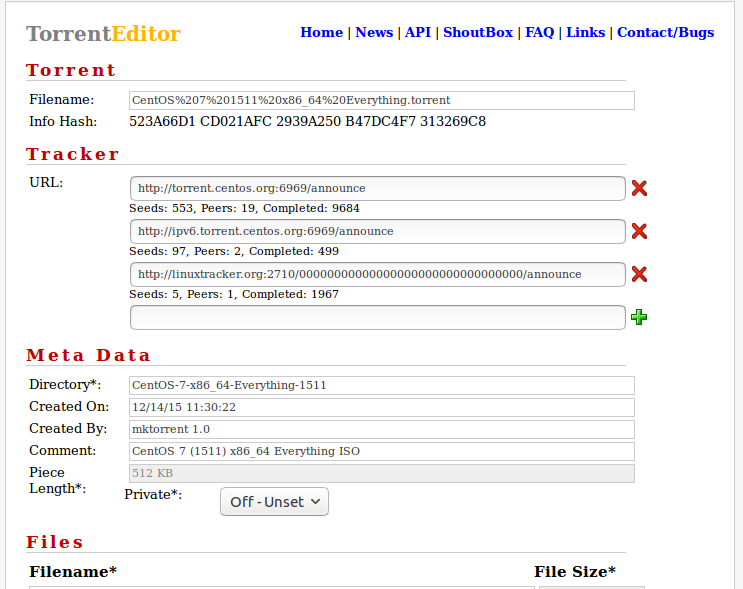
\includegraphics[width=0.7\textwidth]{pics/diffsr.png}
	\caption{Different number of seeders and peers/leechers reported by different trackers.}
	\label{fig:diffsr}
\end{figure}

The \textit{peer translation} receives a list of peers from \textit{libtorrent} and classifies them into seeders and leechers. This procedure is shown in Algorithm \ref{alg:peertrans1}. This algorithm considers \texttt{upload\_only} and \texttt{progress} flags for each peer. To determine whether the peer is a leecher or not, extra flag (\texttt{interested}) is necessary. If the result still zero, the algorithm will consider the downloaded or uploaded amount of that peer from or to the miners. Whichever classification gives the highest number will be picked. Finally, both the projected number of seeders and leechers will be returned to the caller.

\begin{algorithm}[t]
	\caption{Peer translation algorithm}
	\label{alg:peertrans1}
	\begin{adjustwidth}{}{-0.3cm}
	\begin{algorithmic}[1]
	\Function{translate\_peer}{$peer\_list$}
		\State{$num\_seeder \gets 0$}
		\State{$num\_leecher \gets 0$}
		\Statex
		\State{$upload\_only \gets |$\Call{get\_peer}{$UPLOAD\_ONLY$}$|$}
		\State{$finished \gets |$\Call{get\_peer}{$PROGRESS >$ 0.8}$|$}
		\State{$unfinish \gets |$\Call{get\_peer}{$\neg UPLOAD\_ONLY$ \& $PROGRESS < $0.8}$|$}
		\State{$interested \gets |$\Call{get\_peer}{$INTERESTED$}$|$}
		\State $num\_seeder \gets $ \Call{max}{$upload\_only$, $finished$}
		\If{$num\_seeder = 0$}	
		\State $num\_seeder \gets $ number of peer which upload to us $>$ downloaded
		\EndIf
		\State $num\_leecher \gets $ \Call{max}{$interested$, $unfinish$} \label{alg:peertrans1:pickleech}
		\If{$num\_leecher = 0$}	
		\State $num\_leecher \gets $ number of peer which download from us $>$ uploaded
		\EndIf
		\State \Return $num\_seeder$, $num\_leecher$
		\EndFunction
	\end{algorithmic}
	\end{adjustwidth}
\end{algorithm}

\section{Mining stage}
After the prospecting has been done, the mining stage will take place at regular intervals. The mining stage occurs when the credit mining system already has a pool of swarms with potentials. In a fixed interval, the system evaluates the swarms in \textit{swarm selection} algorithm which will be explored in \ref{section:swarmselect}. As a contribution, we proposed a \textit{scoring policy} that will be elaborated more in \ref{section:scorepolicy}.

The credit mining system monitors those swarm continuously. The purpose is to look for swarms that are not performing well in a particular time frame. Under certain requirements, this swarm then will be \textit{stimulated} by optimistically downloading few rare pieces at once. The objective of this approach is to eliminate idleness caused by the bottleneck of share mode. This approach will be elaborated in \ref{section:swarmstimulate}.

\subsection{Swarm Selection}
\label{section:swarmselect}
Swarm selection is the periodic process of selecting swarms based on their mining potential. At some point, the previously selected swarm may not be beneficial anymore and thus needs to be substituted. The swarm selection process is determined by the policy containing rules to sort swarms by their criteria and potential. Currently, all of the miners need to comply with one defined policy.

Three policies have been defined in the preliminary work \cite{2015:creditmining:capota}. Those are based on \textit{Random policy}, \textit{Swarm Age policy}, and \textit{Seeder Ratio policy}. Specifically for \textit{Seeder Ratio policy}, it is specialized to help undersupplied swarms and gave the best credit gain of the three \cite{2015:creditmining:capota}.

\subsection{Scoring Policy}
\label{section:scorepolicy}
The scoring policy is a proposed method to quantify a swarm's prospects and to reduce a possible identical result from two swarms or more. It was brought up with the \textit{seeder ratio policy} as its base. It can be customized with its \textit{score multiplier}.

Scoring policy consists of several elements. The first is the \textit{seeder ratio} which is defined as the ratio of seeders to the total number of peers. The second is the \textit{availability} of a swarm. This represents the piece shortage, which shows the potential to gain more credit for the longer term. The third is the number of peers as a tie-breaker. It is useful to target large swarms instead of small ones as there are comparably more options to give the pieces to. The last is the recent swarm  activity. Inspired by \textit{tit-for-tat}, the policy will prefer a swarm in which any of its peers had interacted with the miners previously.

%Last element that we considered is the activity of a swarm. It is preferable to mine a swarm whose some of the peers already download or upload any data from or to us. Moreover, one which had faster speed is considered. The worst case happened when there is not any peer interested with the piece we already have. In the other hand, if a peer already interacted with us before, there is a chance we will get chosen again in the future. This feature incentivize swarm which had interacted with the miners previously.

\begin{algorithm}[h]
	\caption{Scoring policy algorithm}
	\label{alg:scorep}
	\begin{algorithmic}[1]
		\Require{$M\_leech$ as leecher multiplier}
		\Require{$M\_pratio$ as peer ratio multiplier}
		\Require{$M\_avail$ as peer availability multiplier}
		\Require{$S\_low$ as extra score for lower activity}
		\Require{$S\_high$ as extra score for higher activity}
		\Statex
		\Require{$peerlist$ as the list of stored peers}
		\Require{$swarmlist$ as the list of swarm in the miners}
		\Statex
		\ForAll{$s \in swarmlist$}
			\State{$rleech \gets 1 - $\Call{seeder\_ratio}{s}}
			\State{$rpeer \gets |$\Call{peers}{s}$|/|peerlist|$}
			\State{$ravail \gets 1 - $\Call{availability}{s}$/|peerlist|$}
			\State{$score[s] \gets M\_leech*rleech + M\_pratio * rpeer + M\_avail * ravail$}			\State $total\_speed[s] \gets 0$
			\ForAll{$p \in $\Call{peers}{$s$}}
				\State $total\_speed[s] \gets total\_speed[s] + \Call{get\_speed}{p}$
			\EndFor
		\EndFor
		\State \Call{sort}{$total\_speed$}
		\ForAll{$s \in swarmlist$}
			\If{$index(total\_speed, s) < |total\_speed|/2$}
				\State $score[s] \gets score[s] + S\_low$
			\Else{\null}
				\State $score[s] \gets score[s] + S\_high$
			\EndIf
		\EndFor
		\State \Return{$score$}
	\end{algorithmic}
\end{algorithm}

Scoring policy, as shown in Algorithm \ref{alg:scorep}, starts with examining all of the swarms registered in a miner. Then it decides the score individually as shown in line 2-5. Variable $rpeer$ is the ratio of the number of peers in this swarm to the total number of peers that is already known from all the swarms. \textit{Availability} is the number of complete copies of a piece plus the fraction of the non-seeder peers that provide a subset of a piece. The availability algorithm is explored in Algorithm \ref{alg:savail}. If \textit{availability} is 0, this means that there is not any single piece from any of the discovered peers. It will also return 0 in a case where the piece/peer information could not be received. If all of the peers have a complete files, the \textit{availability} will reach its maximum value which is equal to the number of discovered peers. After the individual score is assigned, the activity of each peer on each of the swarms is calculated. The activity, which we assume as the peer's total download speed to the miner, is sorted in ascending order. Then, the first half of the sorted activity is marked as low activity, and given the lower activity score (line 14). Similarly, this happens with the second half of the list, but with higher activity and a higher score (line 16).

\begin{algorithm}[h]
	\caption{Swarm availability}
	\label{alg:savail}
	\begin{algorithmic}[1]
		\Require{$plist$ as list of stored peers}
		\State $mbit \gets \Call{populate\_piece}{plist}$
		\State $complete\_peer \gets |\Call{get\_seeder}{\null}|$ 
		\State $min\_peer \gets \Call{min}{mbit}$
		\State $more\_piece \gets $ number of piece which has more peer than $min\_peer$
		\State \Return $complete\_peer + min\_peer + more\_peer/|mbit|$
	\end{algorithmic}
\end{algorithm}

The scoring policy is designed in such a way so that it can be easily customized based on user preferences. This can be done by providing value to the following constants: $M\_leech$, $M\_pratio$, $M\_avail$, $S\_low$, and $S\_high$. Changing the multiplier will affect its behavior. For example, if a user does not consider the number of peers to be important, he can set the multiplier for $M\_pratio$ as 0. Setting other parameters except $M\_leech$ as 0 will make scoring policy behave like seeder ratio policy. Similarly, setting other parameters except $M\_avail$ as 0 will prioritize swarm with very low availability. This behavior is similar to if it is applied with swarm age policy in the flashcrowd case.

\subsection{Swarm stimulation}
\label{section:swarmstimulate}
As mentioned in Section \ref{section:sharemode}, activating \textit{share mode} can result in a bottleneck, especially at the start of joining a swarm. \textit{Prospecting} a swarm, if handled correctly, can solve this issue in the prospecting stage itself. By downloading several of the rarest pieces beforehand, the chance that those will be uploaded is high. Therefore, positive upload/download ratio is likely, thus avoiding the \textit{share mode} bottleneck. However, there is not any guarantee when the system is on the mining stage.

We introduced a method to stimulate the mining activity on idle swarms. It starts by looking at which swarms that are already idle for some amount of time. Those swarms are now suspected to be in the \textit{stale} state. We then download several of the rarest pieces on that swarm. We called these pieces the \textit{stimulant}. The stimulant can be downloaded only if the seeder-to-leecher ratio (SLR) for this swarm is higher than the predefined threshold. This threshold should be lower than \texttt{share\_mode\_target} as in both the credit mining system and \textit{libtorrent}. If the ratio is already too low, miners should wait for a piece to be uploaded first. Then, if it is not possible, this swarm will be blacklisted in the next round and be substituted by another swarm. This process is called \textit{stimulating} the swarm. By optimistically download several rarest pieces simultaneously, we hope to stimulate the mining activity in the long term.